\documentclass{beamer}
 
\usepackage[utf8]{inputenc}

\usetheme{Madrid}
\usecolortheme{default}

\usepackage[qm]{qcircuit}
\usepackage{bibentry}
\usepackage{tikz,tikz-cd}

\usepackage{physics}
\usepackage{amsmath}
\usepackage{amsfonts}
\usepackage{esint}
\usepackage{bbold}
\usepackage{caption}
\usepackage{subcaption}
\usepackage{mathtools}
\usepackage{dsfont}
\usepackage{amsthm}
\usepackage{bbm}
\usepackage{amssymb}
\theoremstyle{definition}
\newtheorem{defn}{Definition}[section]
\newtheorem{prop}{Properties}[section]
\newtheorem{rmk}{Remark}[section]
\newtheorem{exmp}{Example}[section]
\newtheorem{prob}{Problem}[section]
\newtheorem{sln}{Solution}[section]
\newtheorem{thm}{Theorem}[section]
\newtheorem*{prob*}{Problem}
\newtheorem*{sln*}{Solution}
\usepackage{empheq}
\usepackage{tensor}
\usepackage{hyperref}
\usepackage{xcolor}

\newcommand{\R}{\mathbb{R}}
\newcommand{\F}{\mathcal{F}}
\newcommand{\p}{\partial}

\newcommand{\V}{\mathbf{V}}
\newcommand{\W}{\mathbf{W}}
\newcommand{\Z}{\mathbf{Z}}
\newcommand{\Y}{\mathbf{Y}}
\newcommand{\U}{\mathbf{U}}
\newcommand{\X}{\mathbf{X}}

\newcommand{\A}{\mathcal{A}}
\newcommand{\B}{\mathcal{B}}

\newcommand{\xpan}{\text{span}}

\newcommand{\lag}{\mathcal{L}}

\newcommand{\J}{\mathbf{J}}

\newcommand{\M}{\mathcal{M}}

\newcommand{\lp}{\left(}
\newcommand{\rp}{\right)}

\newcommand{\lb}{\left[}
\newcommand{\rb}{\right]}

\newcommand{\lc}{\left\{}
\newcommand{\rc}{\right\}}

\newcommand{\K}{\mathcal{K}}

\newcommand{\N}{\mathcal{N}}

\newcommand{\E}{\mathcal{E}}

\newcommand{\ima}{\text{Im}}
\newcommand{\lin}{\overset{\text{linear}}{\longrightarrow}}
\newcommand{\T}{\mathcal{T}}
\newcommand{\poly}{\mathbb{P}}
\newcommand{\s}{\mathcal{S}}
\newcommand{\gives}{\rotatebox[origin=c]{180}{$\Rsh$}	}
\newcommand{\bigzero}{\mbox{\normalfont\Large\bfseries 0}}
\newcommand{\rvline}{\hspace*{-\arraycolsep}\vline\hspace*{-\arraycolsep}}

\title{Measurement-based Quantum Computing \\ \& Efficient variational simulation of non-trivial quantum states}
\author[Huan Q. Bui] % (optional)
{Huan Q. Bui}

\institute[Perimeter Institute] % (optional)
{
	
	Advisor: Timothy Hsieh
	\and
	Perimeter Institute for Theoretical Physics
}
\date{\today}
 
\logo{
\includegraphics[height=1cm]{PI.jpg}}
%
\includegraphics[height=1.3cm]{colby.png}

 
\begin{document}
 
\frame{\titlepage}


%%%%%%%%%%%%%%%%%%%%%%%%%%%%%%%%%%%%%%%%%%%%%%%%%%%%%%%%%%%%%%%%


\begin{frame}

\frametitle{Layout}

\begin{itemize}
	\item Measurement-based quantum computing (MBQC)
	
	\item Variational simulation of non-trivial quantum state
	
	\item \underline{Research question}: MBQC as an efficient simulation?
\end{itemize}

\end{frame}



%%%%%%%%%%%%%%%%%%%%%%%%%%%%%%%%%%%%%%%%%%%%%%%%%%%%%%%%%%%%%%%%


\begin{frame}
\frametitle{MBQC: One-way quantum computer \cite{MBQC}}

Conventional quantum circuit models:

\begin{figure}[!htb]
	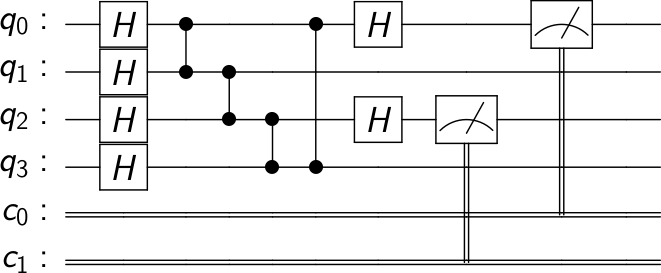
\includegraphics[scale=0.25]{circuit}
\end{figure}

%\pause
Cluster state: \cite{jozsa}

\begin{figure}[!htb]
	%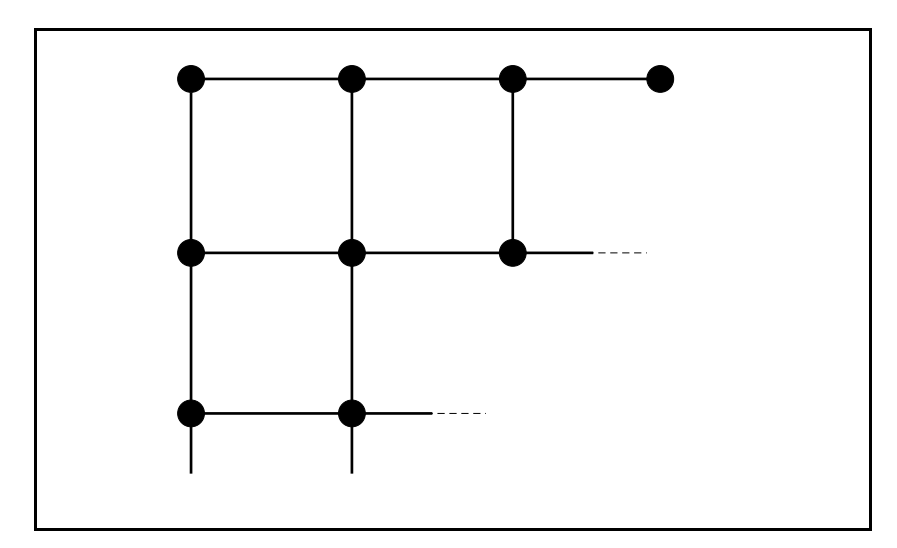
\includegraphics[scale=0.2]{jozsa1}
	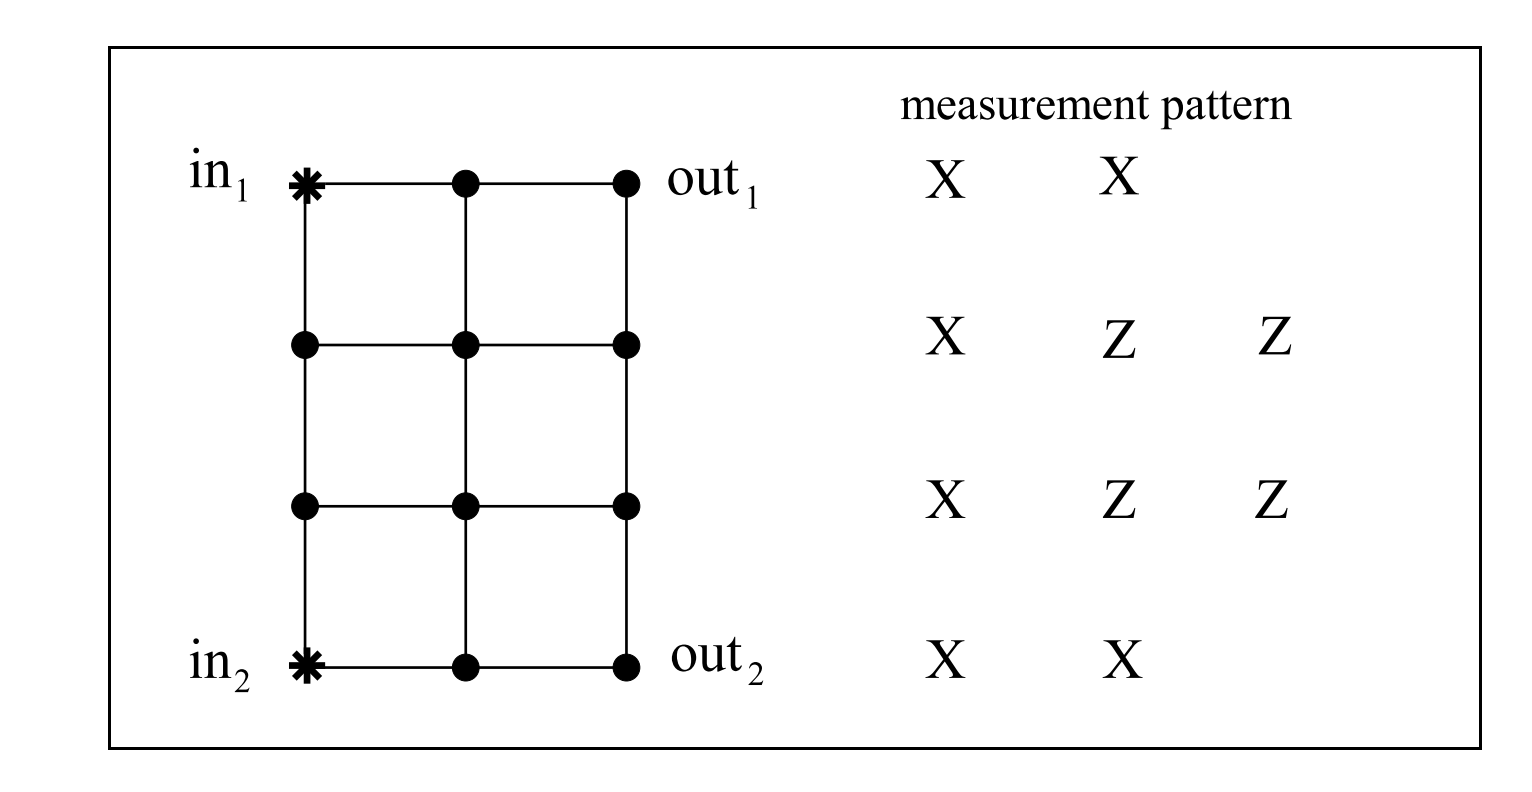
\includegraphics[scale=0.18]{fig8}
\end{figure}







\end{frame}


\begin{frame}[fragile]
\frametitle{MBQC: One-way quantum computer}
Quantum teleportation = Entanglement + Measurement

\begin{center}
	$\,$\Qcircuit @C=.7em @R=1.4em  {
		\lstick{\ket{\psi}} & \qw & \ctrl{1} & \gate{HZ_\theta} & \meter &  \\
		\lstick{\ket{+}}    & \qw & \ctrl{0} & \qw & \qw &\rstick{X^m H Z_\theta \ket{\psi}} 
	}
	
\end{center}

%\pause

\begin{figure}[!htb]
	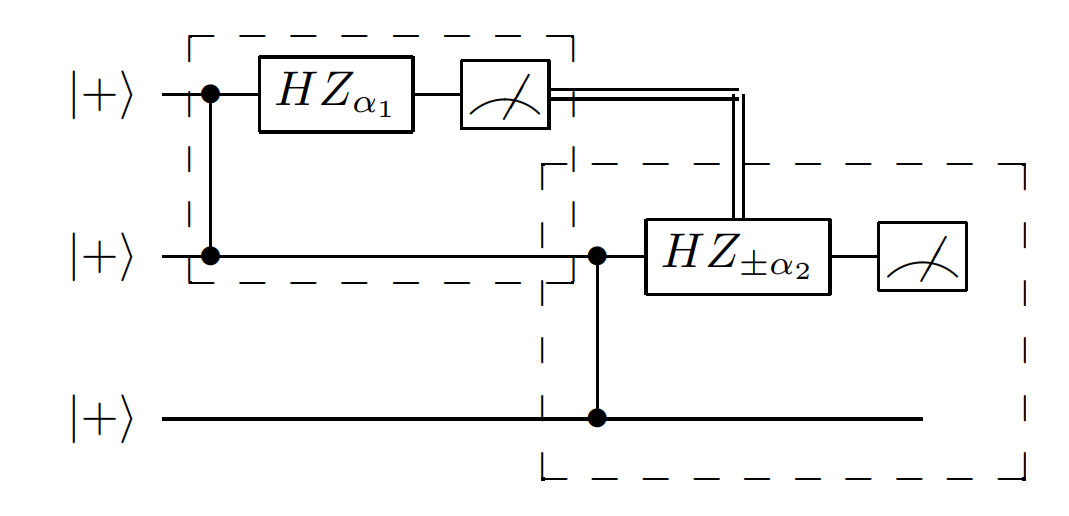
\includegraphics[scale=0.25]{cluster6}
	\caption{From \cite{nielsen}}
\end{figure}


\end{frame}


\begin{frame}
\frametitle{MBQC: One-way quantum computer}

Universality: Quantum circuit model $\equiv$ Cluster state formulation

\begin{itemize}
	\item Transfer of information by teleportation
	\item Any qubit rotation can be done on a chain of qubits
	\item The CNOT gate can be implemented in a ``T'' configuration
\end{itemize}

\begin{figure}[!htb]
	\begin{subfigure}{.5\textwidth}
		\centering
		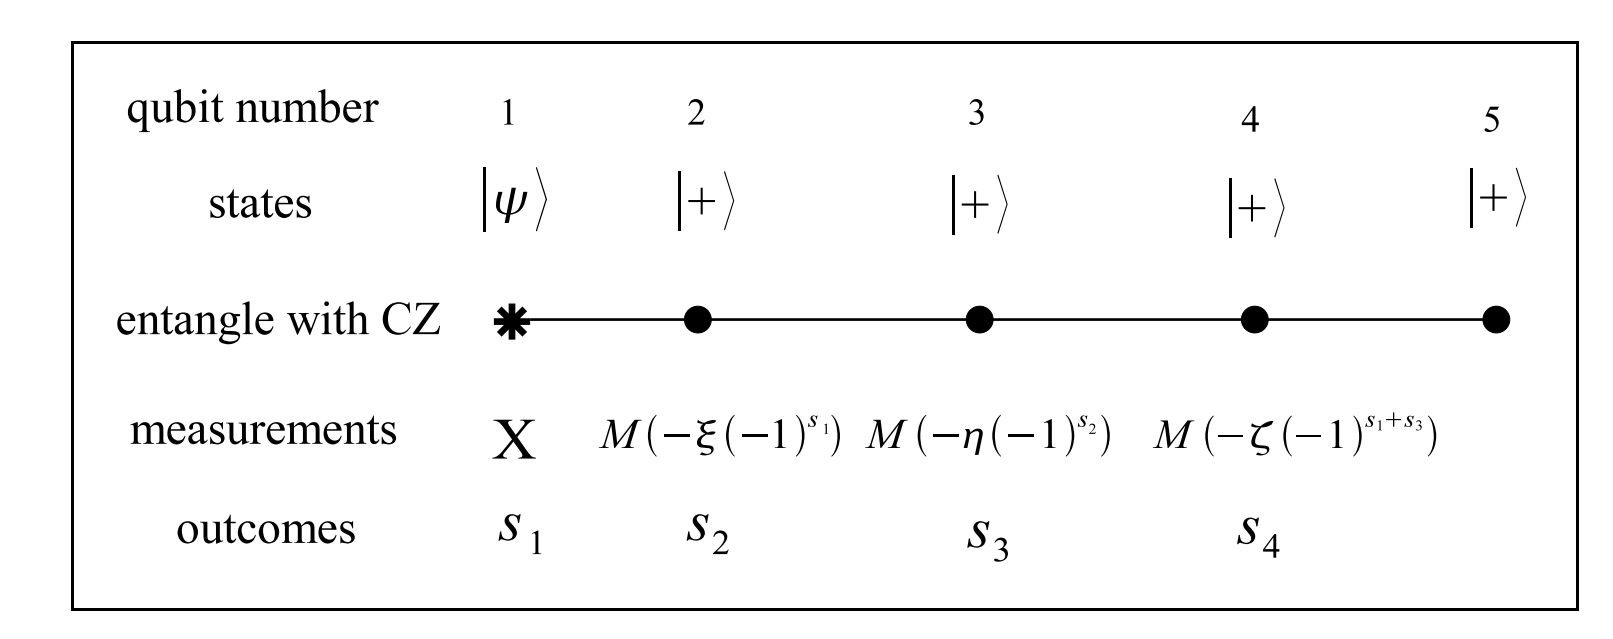
\includegraphics[scale=0.15]{rotate}
		\caption{From \cite{jozsa}}
	\end{subfigure}%
	\begin{subfigure}{.5\textwidth}
		\centering
		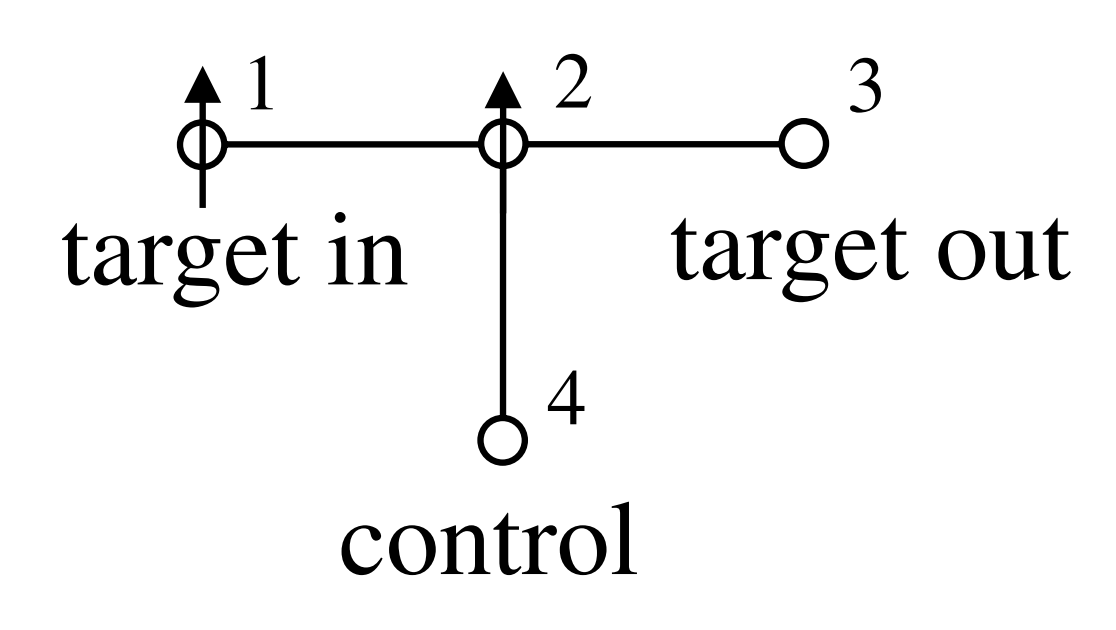
\includegraphics[scale=0.15]{CNOT}
		\caption{From \cite{MBQC}}
	\end{subfigure}
	
	
\end{figure}






\end{frame}
%%%%%%%%%%%%%%%%%%%%%%%%%%%%%%%%%%%%%%%%%%%%%%%%%%%%%%%%%%%%%%%%

\begin{frame}
\frametitle{Variational simulation of non-trivial quantum states}

QAOA:

\end{frame}

%%%%%%%%%%%%%%%%%%%%%%%%%%%%%%%%%%%%%%%%%%%%%%%%%%%%%%%%%%%%%%%%


\begin{frame}
\frametitle{Measurement-based QAOA}



\end{frame}


%%%%%%%%%%%%%%%%%%%%%%%%%%%%%%%%%%%%%%%%%%%%%%%%%%%%%%%%%%%%%%%%


\begin{frame}
\frametitle{Can we do better?}

\end{frame}


%%%%%%%%%%%%%%%%%%%%%%%%%%%%%%%%%%%%%%%%%%%%%%%%%%%%%%%%%%%%%%%%

\begin{frame}
\frametitle{How robust is QAOA?}

Consider the TFIM without translation invariance:

\begin{equation*}
\mathcal{H} = \sum_{j} Z_j Z_{j+1} + \sum_j g_j  X_j
\end{equation*}




\end{frame}



%%%%%%%%%%%%%%%%%%%%%%%%%%%%%%%%%%%%%%%%%%%%%%%%%%%%%%%%%%%%%%%%


\begin{frame}
\frametitle{Summary}



\end{frame}


%%%%%%%%%%%%%%%%%%%%%%%%%%%%%%%%%%%%%%%%%%%%%%%%%%%%%%%%%%%%%%%%


\begin{frame}
\frametitle{References}



\bibliographystyle{amsalpha}
\bibliography{references}{}



\end{frame}










\end{document}